\chapter{Simulations implementation}\label{sec:sim}\thispagestyle{fancy}
%%
The theoretical tool used in this work is the simulation using the transport code ASTRA v.~6.2 (Automated System for TRansport Analysis) \cite{astra}. This allows us to use experimental data as input and modify some parameters, even during the run. It solves 1D radial transport of heat and particles using a set of four flux-surface-averaged diffusive equations. It supports also user-defined additional modules such as additional heating. The equilibrium reconstruction is computed using a 2D fixed-boundary 3-moment equilibrium solver which solves the Grad-Shafranov equation. 

The sawtooth instability can be added to the simulations with the additional package from E. Fable \cite{fableST}. However, this model has been observed to give questionable data in our simulations with density evolution and we decided not to enable the sawteeth to keep the accuracy of the data.

The spatial resolution of the output of ASTRA is not very good since its space-step is $\Delta \rho \sim 0.02$ in our version (ASTRA uses $\rho_{\Phi} = \Phi / \Phi_a$, $\Phi$ being the toroidal magnetic flux). However, the input parameters that define the radial grid are bound to some other parameters, making them very difficult to change without losing the simulation consistency. We were not able to get a better resolution for this work.
%%%%%%%%%% SECTION %%%%%%%%%% {{{1 Temperature computation
\section{Temperature computation}\label{sec:sim:T}
%%
The temperature computation in ASTRA is done with the heat flux. The definition of the heat fluxes implemented in the code have the following form:
\begin{align*}
	\frac{625 q_e}{V' G_1 n_e T_e} & = - \chi^e_n \frac{1}{n_e} \dsd{n_e}{\rho} - \chi_e \frac{1}{T_e} \dsd{T_e}{\rho} - \chi^e_i \frac{1}{T_i} \dsd{T_i}{\rho} + C_e\\
	\frac{625 q_i}{V' G_1 n_i T_i} & = - \chi^i_n \frac{1}{n_e} \dsd{n_e}{\rho} - \chi^i_e \frac{1}{T_e} \dsd{T_e}{\rho} - \chi_i \frac{1}{T_i} \dsd{T_i}{\rho} + C_i
\end{align*}
where $G_1 = \avg{(\nabla \rho)^2}$ and the $\chi_j^k$ are the diffusion coefficients contribution from the other species' temperature or the density to the $k$ species' temperature. As discussed above (\paref{confinement:transport}), the off-diagonal terms are negligible, allowing us to set $\chi^e_i, \chi^i_e, \chi^i_n$ and $\chi^e_n$ to zero in our simulations, as well as $C_e$ and $C_i$.

The electron and ion temperatures are computed using fixed boundary conditions, upon which the whole profile is then built. This implies we must provide consistent data to ASTRA, the better being experimental data. The electron temperature and density are measured using Thomson scattering diagnostic \cite{thomson}. Using these quantities, a few others and some transport scripts, we can build the profiles for every other quantities. But those scripts do not have a good accuracy for H-mode transport since the pedestal steep gradients are not measured precisely enough for them. We must take our ``experimental'' data with a great care if we do not want to provide wrong input to our simulations.

In particular, we have to be careful with the ion temperature, as the said scripts cannot compute it right for H-mode. We can take those data directly from the Charge-eXchange Recombination Spectroscopy (CXRS) measurements. This diagnostic measures specifically the ion temperature \cite{bosshard2003}. Using these data we can have a good ion temperature boundary condition for our simulations.

\begin{wrapfigure}{l}{7cm}
\vspace{-0.5cm}
\includegraphics[width=7cm]{../matlab/pics/a_he.eps}
\vspace{-0.5cm}
\caption{\footnotesize Self-made $\chi_e$ used for H-mode simulations.}
\vspace{-0.5cm}
\end{wrapfigure}
%%
The experimental electron heat diffusivity $\chi_e$ is not available, and the computed one is not accurate. Thus we have to use a self-made $\chi_e$ in the simulation. To achieve this we use a standard L-mode $\chi_e$, i.e. a parabolic one, that we truncate to create the pedestal.

To build an H-mode $\chi_e$, we look for the good L-mode $\chi_e$ without step by running the simulation and changing its profile until the simulated electron temperature presents more or less the same slope as the experimental one, though lower. Then we can truncate this profile to create the pedestal. The temperature pedestal height may be small, but in this work it is important because simulations are implemented such that the density pedestal is computed according to $L_{n_e} \simeq 2 L_{T_e}$ (explained in \paref{sim:n}). Thus to adjust the truncation of $\chi_e$ we try to match the pedestal density profile. To prevent singularities, we do not make a step for the truncation but we use an exponential function to make this step a little smoothed.

To have the energy as near as possible to that given by the scaling law \eqref{eq:confinement:transport:tau_scaling}, we use a scaling on $\chi_e$. During the steady-state phase, we multiply the electron thermal diffusivity by the ratio of the instantaneous energy confinement time divided by the scaling one (see appendix \ref{sec:app:sbr:wscal}). This leads the temperature to what the scaling predicts. To have a little freedom in this procedure, we put a parameter manually modifiable during the simulation, which can be seen as the $H\!H$ factor.

\begin{wrapfigure}{r}{6cm}
\vspace{-9mm}
\includegraphics[width=6cm]{../matlab/pics/40080_0.8_ECHprofile.eps}
\vspace{-7mm}
\caption{\footnotesize ECH power deposition profile.}
\vspace{-5mm}
\end{wrapfigure}
%%
The height of the pedestal of $\chi_e$ is scaled using the same principle as the energy scaling. We use the scaling law \eqref{eq:confinement:Hmode:divertor:WcoreWped} which states that the core energy should be around 3.5 times the pedestal one. We adjust the value of $\chi_e$ in the pedestal region where we have truncated it. This scaling is done during the steady-state standard simulation and is disabled for ELMy simulations.

The ion temperature computation was done using an ASTRA script computing the neoclassical Angioni-Sauter ion heat conductivity \cite{angioni-sauter2000}. As the experimental data are not very good, we cannot determine if there is a pedestal, though the ion temperature should be equal to the electron temperature for $\rho_{\psi} = \sqrt{\psi / \psi_a} > 0.85$ in TCV \cite{andreas2010}. The ion thermal diffusivity was left unchanged for the H-mode simulation.

The ECH power is computed with the TORAY-GA code \cite{matsuda1989}. It is then given to the ASTRA code by the profile of absorption and by the total input power. We thus implement the ECH power as the product of these terms. We must watch this power to stay as it is intended. The total input power is the power integrated over the whole volume. Thus at each time step we renormalize the profile to ensure ourselves that the integrated ECH power remains equal to the experimental injected power.
%% }}}1
%%%%%%%%%% SECTION %%%%%%%%%% {{{1 Density computation
\section{Density computation}\label{sec:sim:n}
%%
The density computation is achieved using the same kind of equation as the temperature computation, the particle flux equation. It is implemented as
\begin{align*}
	\frac{\Gamma_n - \displaystyle\int_0^{\rho} \dd \rho \left( V' S_e - \dsdt{V' n_e} \right)}{V' G_1 n_e} & = - D_n \frac{1}{n_e} \dsd{n_e}{\rho} - \chi^n_e \frac{1}{T_e} \dsd{T_e}{\rho} - \chi^n_i \frac{1}{T_i} \dsd{T_i}{\rho} + V_n
	%\frac{\Gamma_n - \displaystyle\int_0^{\rho} \dd \rho \left( V' S_e - \dsdt{V' n_e} \right)}{V' G_1 n_e} & = - D_n \frac{1}{n_e} \dsd{n_e}{\rho} + V_n
\end{align*}
with $S_e$ the particle source. As discussed above (\paref{confinement:transport}), the off-diagonal terms are contained in $V_n$, thus we set $\chi_e^n, \chi_i^n = 0$. We also do not want any particle source, which is set by $S_e = 0$ for the particle number conservation.

However, ELMs expel particles and energy. The energy is carried by the particles onto the divertor plates. Once there, particles can recombine to form neutral atoms again. If neutral, they are free to move wherever in the vessel, therefore can get back into the plasma and be re-ionized. This yields the density increase right after the ELMs.

Recalling of equation \eqref{eq:confinement:transport:particle:particleFlux}, taking the equilibrium steady-state case means the flux is null and it yields $\nabla n_e / n_e = - V_n / D_n$. We thus have a way to control precisely the density computation through these parameters. It must be noted that the $V_n$ from ASTRA is the opposite of the one we saw in the theory, which yields in ASTRA $\nabla n_e / n_e = V_n / D_n$.

We specify them in such a way that the ratio $V_n / D_n$ is well defined. This is achieved by doing $V_n = a D_n$, so that the ratio is $a$. The diffusion coefficient being a little more free, and according that $D_n \sim 0.2 \chi_e$ in TCV shot with ECH and transport barriers \cite{fable2009}, we set $D_n = 0.2 \chi_e$.

Recalling of \eqref{eq:confinement:Hmode:emil}, we use this scaling linking the density to the temperature for the pedestal region to compute the density. Being unsure about the validity of this scaling, we introduce a free parameter to be able to adjust our profile. The density peaking $n_{e,0} / \avg{n_e}$ gives us information about the gradient length for the density. Having a highly peaked profile we understand the gradient length $L_n$ associated is small. The profile peaking values for TCV SN shots may be in the range 1 -- 1.4 \cite{andreas2010}. This allows us to give ASTRA a value around the unity for the ratio $V_n / D_n$ for the core region.

In summary, once the values of $n_e( \rho = 1 )$, $T_e( \rho = 1 )$ and $T_i( \rho = 1 )$ are given, the profiles are determined by the following assumptions (except if stated otherwise):
\begin{itemize}
	\item $\chi_e \sim \rho^2$ in the core
	\item $\tau_E = H\!H\ \tau_{\mathrm{IPB}98(y,2)}$
	\item $W_{core} = 3.5\ W_{ped}$ acting on $\chi_e$ in the pedestal region
	\item $D = 0.2\ \chi_e$ in the core
	\item $\nabla n_e / n_e = 0.5\ \nabla T_e / T_e$ in the pedestal region
\end{itemize}

%% }}}1
%%%%%%%%%% SECTION %%%%%%%%%% {{{1 ELM implementation
\section{ELM implementation}\label{sec:sim:ELM}
%%
The ELMs were not triggered in the simulations from MHD instabilities as explained above (\paref{MHD:instab}), but done manually. They were achieved by modifying the profile of $\chi_e$, $\chi_i$ and $D_n$ radically. Increasing these transport coefficients by many orders of magnitude at the edge, this means the edge transport is very important and therefore the profiles flatten near the edge while keeping the boundary value fixed to the imposed value. This mimics an unstable mode which would be localized near the edge.

The profiles for $\chi$ and $D_n$ are shown below. The density diffusivity was raised less because its pedestal has been observed to decrease less in experiments with type-I ELMs \cite{andreas2010}.

\begin{figure}[H]
\vspace{-2mm}
\begin{center}
\subfloat[]{\includegraphics[width=5cm]{../matlab/pics/a_he_ELM.eps}\label{fig:sim:ELM:chiDnELM:chi}}
\hspace{3mm}
\subfloat[]{\includegraphics[width=5cm]{../matlab/pics/a_dn_ELM.eps}\label{fig:sim:ELM:chiDnELM:dn}}
\vspace{-7mm}
\end{center}
\caption{\footnotesize $\chi$ and $D_n$ used to create the ELMs.\label{fig:sim:ELM:chiDnELM}}
\vspace{-5mm}
\end{figure}

The ELM ``standard parameters'' for our simulations are a duration of $\tauELM\mu s$ and a frequency of $\fELM Hz$ (experimental data), the changes have a radial interaction range of the temperature pedestal range (approximately $0.78 < \rho_{\Phi} < 1$), and an amplitude of $10'000\ m^2 s^{-1}$ in $\chi_e$ and $\chi_i$ and of $20\ m^2 s^{-1}$ in $D_n$. This choice was made to have the temperature pedestal fully flattened by the ELM. The density pedestal has been observed to be slower to be destroyed \cite{andreas2010}. The choice of the $20\ m^2 s^{-1}$ has been made to reproduce this behavior. However, the experiment ELM expelled energy was higher than what we got in our simulations. We tried to increase this value, but the density pedestal flattened much faster than the expelled energy increased. It was thus chosen to let this arbitrary value to keep the desired behavior of the density pedestal during the ELM.

The registered ELM was the eleventh one, but we also saved the first one of the same simulation to compare them together in further analysis. As can be seen on the time trace of the thermal diffusivity~\figref{sim:ELM:chie_trace}, we set the simulation time to be at $t = 0$ at the onset of the ELM. Then the ELM stops at $t = 0.1ms$ and the next one starts at $t = 20ms$.

\begin{figure}[H]
\vspace{-2mm}
\begin{center}
\subfloat[\footnotesize $D_{\alpha}$ time trace showing the ELM crash.]{\includegraphics[width=5cm]{../matlab/pics/40080_Da.eps}}%\label{fig:##}}
\hspace{3mm}
\subfloat[\footnotesize Time trace of $\chi_e$. $\chi_i$ is the same, and $D_n$ is like this one but not as high during the ELM.]{\includegraphics[width=5cm]{../matlab/pics/40080_0.8_chie_trace.eps}\label{fig:sim:ELM:chie_trace}}
\vspace{-8mm}
\end{center}
\caption{\footnotesize ELM experimental and simulation time traces.}%\label{fig:##}}
\vspace{-5mm}
\end{figure}
%%
%% }}}1
